\listfiles

\documentclass[a4paper,ngerman,12pt,bibtotoc]{scrartcl}

\usepackage[utf8]{inputenc}

\usepackage[ngerman]{babel}
\addto\captionsngerman{\renewcommand\tablename{Tafel}}

\usepackage{amsmath, amsthm, amssymb, stmaryrd, color, graphicx, mathtools}
\usepackage{setspace}
\usepackage{bussproofs}
\usepackage{array}
\usepackage{booktabs}
\usepackage{comment}
\usepackage{textcomp}
\usepackage{stmaryrd}

\usepackage[protrusion=true,expansion=true]{microtype}

\usepackage{lmodern}
\usepackage{tabto}

\usepackage[backend=bibtex,style=alphabetic]{biblatex}
\usepackage[babel]{csquotes}
\bibliography{literatur}

\usepackage{titling}

\usepackage[all]{xy}

\usepackage[colorlinks=true, linkcolor=blue, urlcolor=blue, citecolor=blue]{hyperref}
\usepackage{cleveref}			%Referenzen mit Name


\usepackage{algorithm}
\usepackage{algpseudocode}
\algrenewcommand{\algorithmiccomment}[1]{\hskip3em$\slash\slash$ #1}
\newcommand{\LineFor}[2]{\State\algorithmicfor\ {#1}\ \algorithmicdo\ {#2} \algorithmicend\ \algorithmicfor}


\setlength\parskip{\medskipamount}
\setlength\parindent{0pt}

\theoremstyle{definition}
\newtheorem{defn}{Definition}[section]
\newtheorem{axiom}[defn]{Axiom}
\newtheorem{bsp}[defn]{Beispiel}

\theoremstyle{plain}

\newtheorem{prop}[defn]{Proposition}
\newtheorem{motto}[defn]{Motto}
\newtheorem{ueberlegung}[defn]{Überlegung}
\newtheorem{lemma}[defn]{Lemma}
\newtheorem{kor}[defn]{Korollar}
\newtheorem{hilfsaussage}[defn]{Hilfsaussage}
\newtheorem{satz}[defn]{Satz}

\theoremstyle{remark}
\newtheorem{erin}[defn]{Erinnerung}
\newtheorem{bem}[defn]{Bemerkung}
\newtheorem{beob}[defn]{Beobachtung}
\newtheorem{aufg}[defn]{Aufgabe}

\clubpenalty=10000
\widowpenalty=10000
\displaywidowpenalty=10000

\newcommand{\ZZ}{\mathbb{Z}}
\newcommand{\QQ}{\mathbb{Q}}
\newcommand{\RR}{\mathbb{R}}
\newcommand{\CC}{\mathbb{C}}
\newcommand{\NN}{\mathbb{N}}
\newcommand{\PP}{\mathbb{P}}
\newcommand{\Ic}{\mathcal{I}}
\newcommand{\Jc}{\mathcal{J}}
\newcommand{\Hc}{\mathcal{H}}
\newcommand{\Tc}{\mathcal{T}}
\newcommand{\Sc}{\mathcal{S}}
\newcommand{\Oc}{\mathcal{O}}


\newcommand{\Hom}{\mathrm{Hom}}
\newcommand{\id}{\mathrm{id}}
\newcommand{\Id}{\mathrm{Id}}

\newcommand{\OPT}{\mathrm{OPT}}
\newcommand{\MST}{\mathrm{MST}}

\newcommand{\HetTSP}{\textsc{HetTSP}}
\newcommand{\HetCVRP}{\textsc{HetCVRP}}


\renewcommand*\theenumi{\alph{enumi}}
\renewcommand{\labelenumi}{(\theenumi)}

\setcounter{tocdepth}{2}

\newenvironment{indentblock}{%
	\list{}{\leftmargin\leftmargin}%
	\item\relax
}{%
\endlist
}



\begin{document}
	\author{Lukas Graf}
	\date{Letzte Aktualisierung: \today}
	
	\selectlanguage{ngerman}
	\thispagestyle{empty}
	
	
	\begin{titlepage}\center
	\textsc{\LARGE Universität Augsburg}\\[1.5cm]
	
	\textsc{\Large Institut für Mathematik}\\[2.5cm]
	
	% Title
	{\Large Seminar\glqq ausarbeitung\grqq \\[1cm]}
	zu einem Vortrag im Seminar Spieltheorie und Approximationsalgorithmen im SS 2016 zum Thema\\[1.5cm]
	{\huge Capacitated Vehicle Routing with Non-Uniform Speeds}
		
	
	\vfill
	
	% Author and supervisor
	\begin{minipage}{0.4\textwidth}
		\begin{flushleft} \large
			\emph{Zusammengestellt:}\\
			Lukas \textsc{Graf}
		\end{flushleft}
	\end{minipage}
	\begin{minipage}{0.4\textwidth}
		\begin{flushright} \large
			\emph{Betreut von:} \\
			M. Sc. Manuel \textsc{Surek},\\Prof. Dr. Tobias \textsc{Harks}
		\end{flushright}
	\end{minipage}
	
	\end{titlepage}
	
	\section{Problemübersicht}
	
		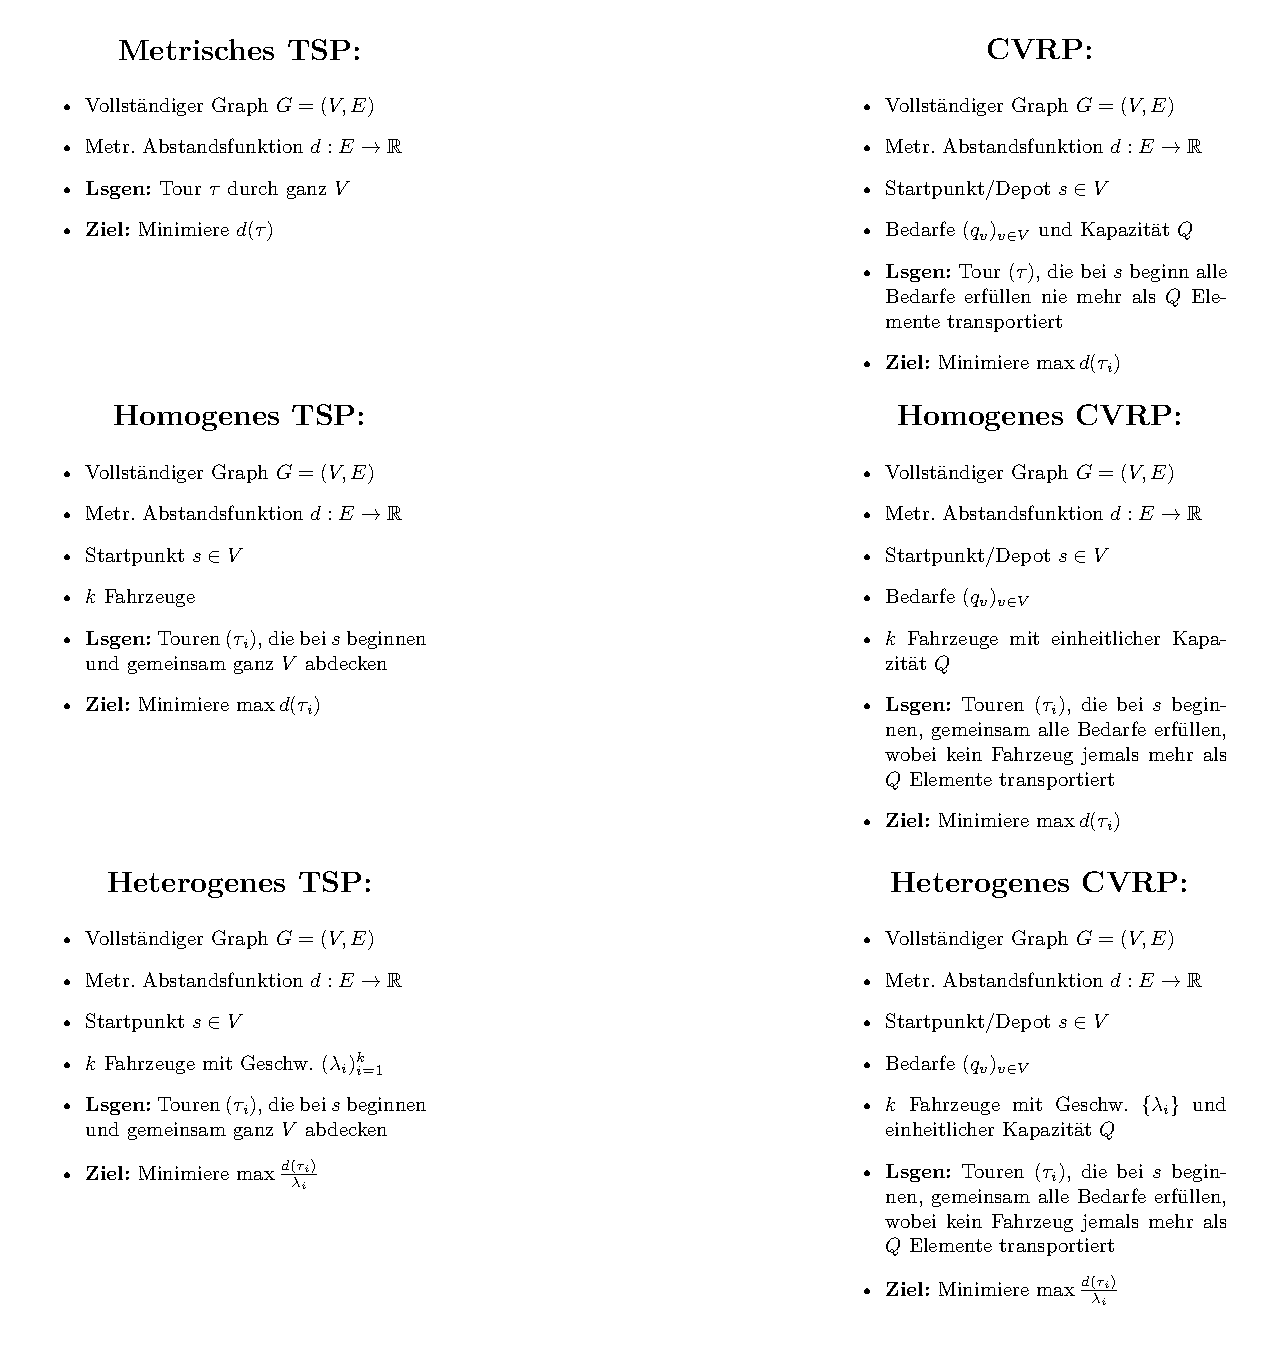
\includegraphics[width=1\textwidth]{Problemdefinitionen.pdf}
	
	\newpage
	\section{Algorithmus für \HetTSP}
	
	\begin{algorithm}[H]
		\caption{HetTSP-Approx}\label{AlgHetTSP}
		\begin{algorithmic}[1]
			\Procedure{HetTSP}{$G=(V,E)$, $d:E\to \RR_{\geq 0}$}
			\State Rate $M$ mit $\frac{M}{2} \leq \OPT \leq M$
			\State $\Hc := \left(H_i\right)_{i\geq 0} \gets$ \textsc{Level-Prime} $\left(G, d\right)$
			\Statex \Comment{$\Hc$ erfüllt: Wurzel-Blatt Pfade haben aufsteigende Knoten-Level}
			\Statex \Comment{\phantom{$\Hc$ erfüllt:} und $\forall i: \sum_{j\geq i}d\left(H_j\right)\leq 8 M \sum_{j\geq i-1}2^j\mu_j$ (wenn $M$ korrekt geraten)}
			\State $\Tc := \left(\Tc_i\right)_{i\geq 0} \gets$ \textsc{Decomposition} $\left(\Hc\right)$
			\Statex \Comment{$\Tc$ ist $\left(6, 40\right)$-zuweisbarer Wald}
			\State $\left(x_{ij}\right) \gets$ \textsc{FractionalAssignment}  $\left(\Tc\right)$
			\State $\left(\tau_i\right) \gets$ \textsc{RoundingAssignment} $\left(x_{ij}\right)$
			\Statex \Comment{$\Tc$ ist $\left(\alpha, \beta\right)$-zuweisbar $\Rightarrow$ $\left(\tau_i\right)$ ist $\left(4\alpha+2\beta\right)$-approx.}
			\State \Return $\left(\tau_i\right)$
			\EndProcedure
		\end{algorithmic}
	\end{algorithm}
	
	\begin{satz}[Theorem 1.1 in \cite{HetCVRP}]
		\Cref{AlgHetTSP} ist ein $\Oc(1)$-approximativer Algorithmus für \HetTSP.
	\end{satz}
	
	\subsection{Level-Prime}
	
	\begin{algorithm}[H]
		\caption{Level-Prime}\label{AlgLevelPrime}
		\begin{algorithmic}[1]
			\Procedure{Level-Prime}{$G=(V,E)$, $d:E\to \RR_{\geq 0}$}
			\State $V_0 := \left\lbrace v\in V \mid d(s,v) \leq M\right\rbrace,\quad V_i := \left\lbrace v \in V \mid 2^{i-1}M < d(s,v) \leq 2^i M\right\rbrace$
			\LineFor{$i\geq 0$}{$H_i \gets$ Minimaler Spannbaum auf $G\left[V_{\leq i}\right]/V_{<i}$}
			\State \Return $\left(H_i\right)_{i\geq 0}$
			\EndProcedure
		\end{algorithmic}
	\end{algorithm}	
	
	\begin{lemma}[Theorem 3.3 in \cite{HetCVRP}]
		Ein von \cref{AlgLevelPrime} gefundener Baum $\left(H_l\right)_{l\geq 0}$ erfüllt:
		\begin{itemize}
			\item Die Knoten-Level entlang jedes Wurzel-Blatt-Pfades sind monoton wachsend.
			\item $\forall k\geq 0: \sum_{l\geq k} d(H_l) \leq 8\cdot \MST(G/V_{<k})$
		\end{itemize}
	\end{lemma}
	
	\begin{kor}[Korollar 3.5 in \cite{HetCVRP}]
		Ein von \cref{AlgLevelPrime} gefundener Baum $\left(H_l\right)_{l\geq 0}$ erfüllt:
		\begin{itemize}
			\item Die Knoten-Level entlang jedes Wurzel-Blatt-Pfades sind monoton wachsend.
			\item $\forall k\geq 1: \sum_{l>k} d(H_l) \leq 8\cdot \sum_{l\geq k}2^l\mu_l$
		\end{itemize}
	\end{kor}
	
	
	\subsection{Decomposition-Algorithmus}
	
	\begin{algorithm}[H]
		\caption{Decomposition}\label{AlgDecomposition}
		\begin{algorithmic}[1]
			\Procedure{Decomposition}{$\left(\Hc\right)$}
			\State $\Sc_0 := \left\lbrace H_0 \right\rbrace,\quad \Sc_i := \text{Zerl. von } \Hc\cap E_i \text{ in Bäume mit genau einer Kante nach } V_i$
			\State 
			\State \Return $\left(\Tc_i\right)_{i\geq 0}$
			\EndProcedure
		\end{algorithmic}
	\end{algorithm}
	
	\begin{defn}[Definition 3.1 in \cite{HetCVRP}]
		Ein Wald $\Tc = \bigcup_{l\geq 0} \Tc_l$ aus Bäumen mit Wurzel $s$ heißt $(\alpha, \beta)$-zuweisbar, wenn gilt:
		\begin{itemize}
			\item Für alle $T \in \Tc_l$ gilt: $d(T) \leq \alpha 2^l M$ \\
			\textit{d.h. ein Baum aus $\Tc_l$ kann mit Geschw. $2^l$ in $\Oc(\alpha M)$ besucht werden.}
			\item Für alle $k \geq 1$ gilt: $\sum_{l > k} d(\Tc_l) \leq \beta M \sum_{l\geq k} 2^l\mu_l$
			
			\textit{d.h. die Fahrzeuge mit Geschw. $\geq 2^k$ können den Wald $\Tc_{>k}$ in $\Oc(\beta M)$ besuchen.}
		\end{itemize}
	\end{defn}
	
	\begin{lemma}[Lemma 3.11 in \cite{HetCVRP}]
		Die von \cref{AlgDecomposition} bestimmte Zerlegung $\Tc = (\Tc_i)_{i\geq 0}$ ist $(6, 40)$-zuweisbar.
	\end{lemma}
	
	
	\subsection{Assignment-Algorithmen}

	\begin{algorithm}[H]
		\caption{FractionalAssignment}\label{AlgFractionalAssignment}
		\begin{algorithmic}[1]
			\Procedure{FractionalAssignment}{$\left(\Tc\right)$}
			\State 
			\State \Return $\left(x_{ij}\right)$
			\EndProcedure
		\end{algorithmic}
	\end{algorithm}
	
	\begin{prop}[Seite 54 (?) in \cite{bMatching}]
		
	\end{prop}
	
	\begin{algorithm}
		\caption{RoundingAssignment}\label{AlgRoundingAssignment}
		\begin{algorithmic}[1]
			\Procedure{RoundingAssignment}{$\left(x_{ij}\right)$}
			\State 
			\State \Return $\left(\tau_i\right)$
			\EndProcedure
		\end{algorithmic}
	\end{algorithm}
	
	\begin{prop}[Theorem 1 in \cite{Rounding}]
		
	\end{prop}
	
	\begin{lemma}[Lemma 3.2 in \cite{HetCVRP}]
		Gegeben einen $(\alpha, \beta)$-zuweisbaren Wald, liefern \cref{AlgFractionalAssignment} und \cref{AlgRoundingAssignment} eine $(4\alpha+2\beta)$-approximative Lösung für \HetTSP.
	\end{lemma}
	
	
	\section{Algorithmus für \HetCVRP}
	
	\begin{satz}[Theorem 4.1 in \cite{HetCVRP}]
		Es gibt eine $\Oc(1)$-approximationserhaltende Reduktion von \HetTSP{} auf \HetCVRP.
	\end{satz}

	\newpage
	\nocite{*}
	\printbibliography		
			
\end{document}